\documentclass[tikz,border=10pt]{standalone}
\usetikzlibrary{arrows.meta}
\begin{document}
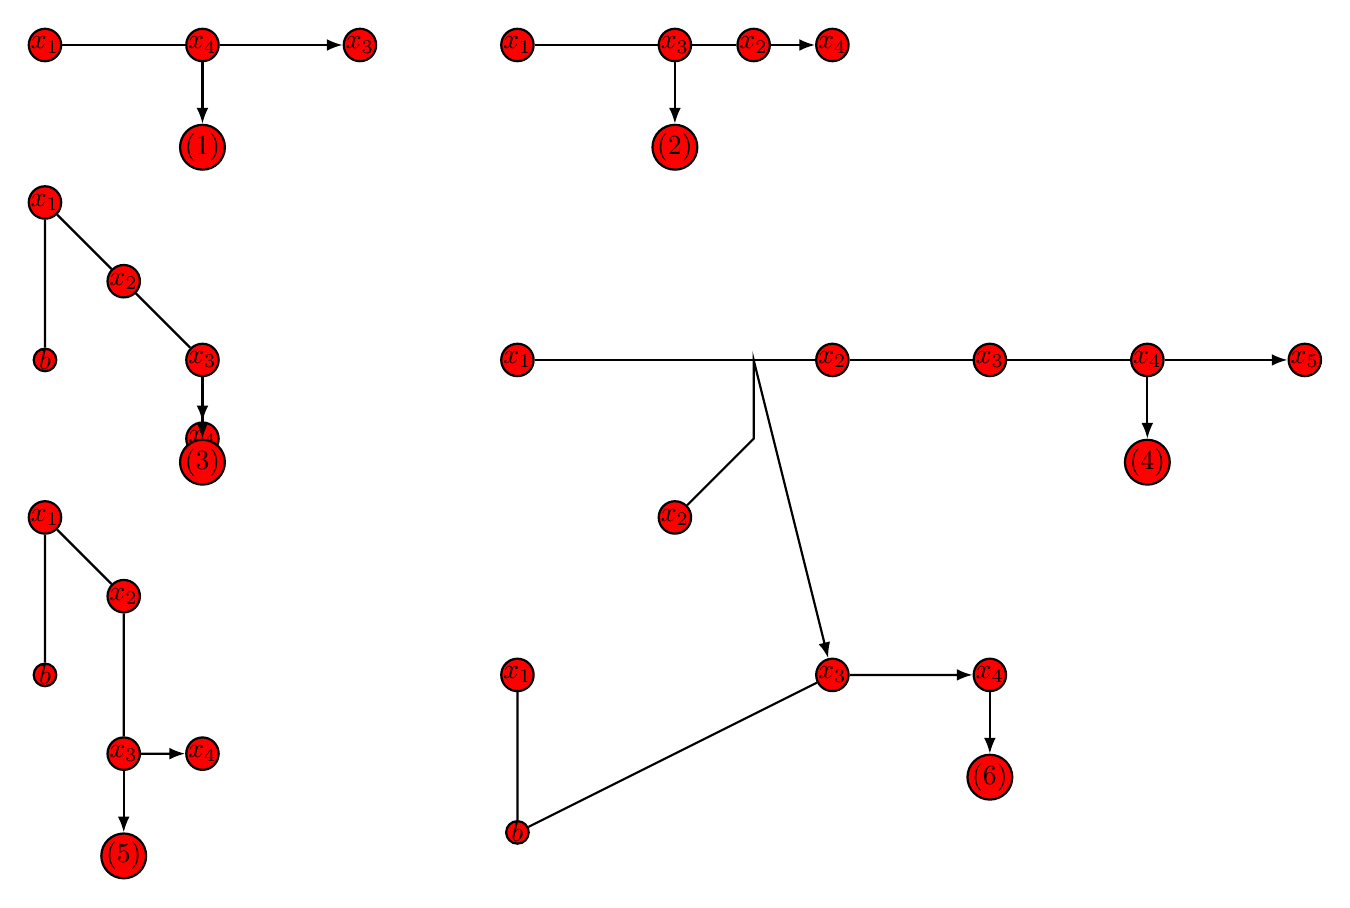
\begin{tikzpicture}[
  every node/.style={draw, circle, fill=red, minimum size=2mm, inner sep=0pt},
  every path/.style={thick, -{Latex[length=2mm, width=1.5mm]}}
]

% Tree 1
\begin{scope}[xshift=0cm]
  \node (x1) at (0,0) {$x_1$};
  \node (x4) at (2,0) {$x_4$};
  \node (x3) at (4,0) {$x_3$};
  \draw (x1) -- (x4) -- (x3);
  \draw (x4) -- ++(0,-1) node[below] {(1)};
\end{scope}

% Tree 2
\begin{scope}[xshift=6cm]
  \node (x1) at (0,0) {$x_1$};
  \node (x3) at (2,0) {$x_3$};
  \node (x2) at (3,0) {$x_2$};
  \node (x4) at (4,0) {$x_4$};
  \draw (x1) -- (x3) -- (x2) -- (x4);
  \draw (x3) -- ++(0,-1) node[below] {(2)};
\end{scope}

% Tree 3
\begin{scope}[xshift=0cm, yshift=-4cm]
  \node (b) at (0,0) {$b$};
  \node (x2) at (1,1) {$x_2$};
  \node (x1) at (0,2) {$x_1$};
  \node (x4) at (2,-1) {$x_4$};
  \node (x3) at (2,0) {$x_3$};
  \draw (b) -- (x1) -- (x2) -- (x3) -- (x4);
  \draw (x3) -- ++(0,-1) node[below] {(3)};
\end{scope}

% Tree 4
\begin{scope}[xshift=6cm, yshift=-4cm]
  \node (x1) at (0,0) {$x_1$};
  \node (x5) at (10,0) {$x_5$};
  \node (x4) at (8,0) {$x_4$};
  \node (x3) at (6,0) {$x_3$};
  \node (x2) at (4,0) {$x_2$};
  \draw (x1) -- (x2) -- (x3) -- (x4) -- (x5);
  \draw (x4) -- ++(0,-1) node[below] {(4)};
\end{scope}

% Tree 5
\begin{scope}[xshift=0cm, yshift=-8cm]
  \node (b) at (0,0) {$b$};
  \node (x2) at (1,1) {$x_2$};
  \node (x1) at (0,2) {$x_1$};
  \node (x4) at (2,-1) {$x_4$};
  \node (x3) at (1,-1) {$x_3$};
  \draw (b) -- (x1) -- (x2) -- (x3) -- (x4);
  \draw (x3) -- ++(0,-1) node[below] {(5)};
\end{scope}

% Tree 6
\begin{scope}[xshift=6cm, yshift=-8cm]
  \node (x1) at (0,0) {$x_1$};
  \node (x2) at (2,2) {$x_2$};
  \node (x4) at (6,0) {$x_4$};
  \node (b) at (0,-2) {$b$};
  \node (x3) at (4,0) {$x_3$};
  \draw (x1) -- (b) -- (x3) -- (x4);
  \draw (x2) -- ++(1,1) -- ++(0,1) -- (x3);
  \draw (x4) -- ++(0,-1) node[below] {(6)};
\end{scope}

\end{tikzpicture}
\end{document}